\documentclass[tikz,border=10pt]{standalone}
\usetikzlibrary{positioning, fit, backgrounds, calc}

\begin{document}
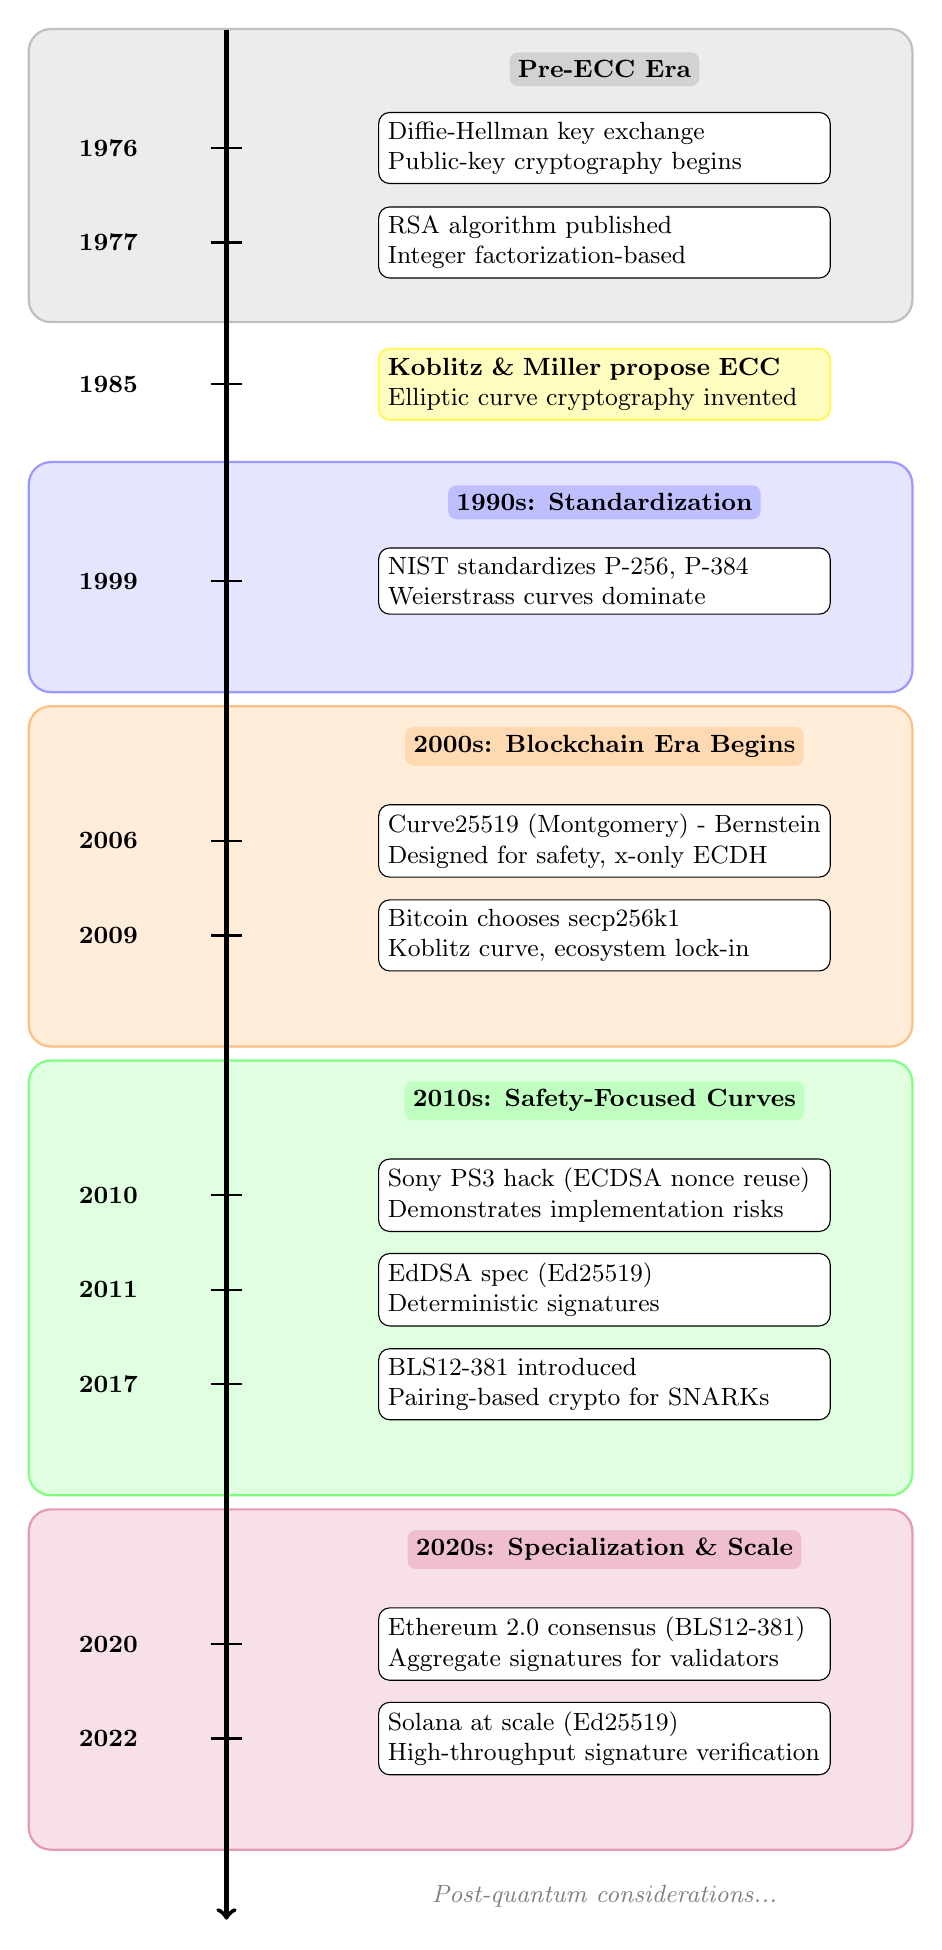
\begin{tikzpicture}[
  year/.style={minimum size=0.8cm, font=\small\bfseries},
  event/.style={rectangle, draw, rounded corners, fill=white, text width=5.5cm, align=left, minimum height=0.8cm, font=\small},
  eralabel/.style={font=\small\bfseries, fill=white, draw=none, rounded corners=3pt, inner sep=3pt},
  % Era box styles with distinct colors
  preecc/.style={rounded corners=8pt, fill=gray!15, draw=gray!50, thick},
  era90s/.style={rounded corners=8pt, fill=blue!10, draw=blue!40, thick},
  era00s/.style={rounded corners=8pt, fill=orange!15, draw=orange!50, thick},
  era10s/.style={rounded corners=8pt, fill=green!12, draw=green!50, thick},
  era20s/.style={rounded corners=8pt, fill=purple!12, draw=purple!40, thick}
]

% Timeline axis - centered at x=0
\draw[ultra thick, ->] (0,4.5) -- (0,-19.5);

% Tick marks on the timeline
\foreach \y in {3, 1.8, 0, -2.5, -5.8, -7, -10.3, -11.5, -12.7, -16, -17.2} {
  \draw[thick] (-0.2, \y) -- (0.2, \y);
}

% ============================================
% PRE-ECC ERA (before 1985)
% ============================================
\begin{scope}[on background layer]
  \node[preecc, fit={(-2.3,4.3) (8.5,1)}, inner sep=6pt] (preerabox) {};
\end{scope}
\node[eralabel, fill=gray!35] at (4.8, 4) {Pre-ECC Era};

\node[year] at (-1.5, 3) {1976};
\node[event] at (4.8, 3) {Diffie-Hellman key exchange\\Public-key cryptography begins};

\node[year] at (-1.5, 1.8) {1977};
\node[event] at (4.8, 1.8) {RSA algorithm published\\Integer factorization-based};

% ============================================
% ECC BIRTH (1985)
% ============================================
\node[year] at (-1.5, 0) {1985};
\node[event, fill=yellow!25, draw=yellow!60, thick] at (4.8, 0) {\textbf{Koblitz \& Miller propose ECC}\\Elliptic curve cryptography invented};

% ============================================
% 1990s ERA - Standardization
% ============================================
\begin{scope}[on background layer]
  \node[era90s, fit={(-2.3,-1.2) (8.5,-3.7)}, inner sep=6pt] (era90box) {};
\end{scope}
\node[eralabel, fill=blue!25] at (4.8, -1.5) {1990s: Standardization};

\node[year] at (-1.5, -2.5) {1999};
\node[event] at (4.8, -2.5) {NIST standardizes P-256, P-384\\Weierstrass curves dominate};

% ============================================
% 2000s ERA - Blockchain Begins
% ============================================
\begin{scope}[on background layer]
  \node[era00s, fit={(-2.3,-4.3) (8.5,-8.2)}, inner sep=6pt] (era00box) {};
\end{scope}
\node[eralabel, fill=orange!30] at (4.8, -4.6) {2000s: Blockchain Era Begins};

\node[year] at (-1.5, -5.8) {2006};
\node[event] at (4.8, -5.8) {Curve25519 (Montgomery) - Bernstein\\Designed for safety, x-only ECDH};

\node[year] at (-1.5, -7) {2009};
\node[event] at (4.8, -7) {Bitcoin chooses secp256k1\\Koblitz curve, ecosystem lock-in};

% ============================================
% 2010s ERA - Safety Focus
% ============================================
\begin{scope}[on background layer]
  \node[era10s, fit={(-2.3,-8.8) (8.5,-13.9)}, inner sep=6pt] (era10box) {};
\end{scope}
\node[eralabel, fill=green!25] at (4.8, -9.1) {2010s: Safety-Focused Curves};

\node[year] at (-1.5, -10.3) {2010};
\node[event] at (4.8, -10.3) {Sony PS3 hack (ECDSA nonce reuse)\\Demonstrates implementation risks};

\node[year] at (-1.5, -11.5) {2011};
\node[event] at (4.8, -11.5) {EdDSA spec (Ed25519)\\Deterministic signatures};

\node[year] at (-1.5, -12.7) {2017};
\node[event] at (4.8, -12.7) {BLS12-381 introduced\\Pairing-based crypto for SNARKs};

% ============================================
% 2020s ERA - Specialization
% ============================================
\begin{scope}[on background layer]
  \node[era20s, fit={(-2.3,-14.5) (8.5,-18.4)}, inner sep=6pt] (era20box) {};
\end{scope}
\node[eralabel, fill=purple!25] at (4.8, -14.8) {2020s: Specialization \& Scale};

\node[year] at (-1.5, -16) {2020};
\node[event] at (4.8, -16) {Ethereum 2.0 consensus (BLS12-381)\\Aggregate signatures for validators};

\node[year] at (-1.5, -17.2) {2022};
\node[event] at (4.8, -17.2) {Solana at scale (Ed25519)\\High-throughput signature verification};

% Future arrow indicator
\node[font=\small\itshape, text=gray] at (4.8, -19.2) {Post-quantum considerations...};

\end{tikzpicture}
\end{document}
